\chapter{درخت‌های فراگیر}

\index{درخت فراگیر}

یک \key{درخت فراگیر} از یک گراف شامل تمام رأس‌های گراف و تعدادی از یال‌های آن است، به طوری که بین هر دو رأس یک مسیر وجود داشته باشد.
مانند درخت‌ها به طور کلی، درخت‌های فراگیر همبند و بدون دور هستند.
معمولاً چندین روش برای ساخت یک درخت فراگیر وجود دارد.

برای مثال، گراف زیر را در نظر بگیرید:
\begin{center}
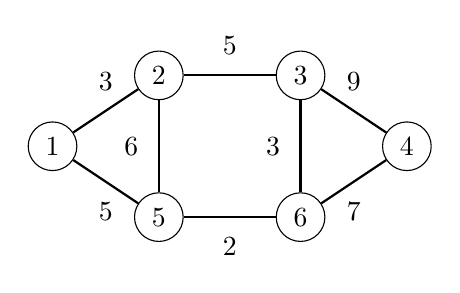
\begin{tikzpicture}[scale=0.9]
\node[draw, circle] (1) at (1.5,2) {$1$};
\node[draw, circle] (2) at (3,3) {$2$};
\node[draw, circle] (3) at (5,3) {$3$};
\node[draw, circle] (4) at (6.5,2) {$4$};
\node[draw, circle] (5) at (3,1) {$5$};
\node[draw, circle] (6) at (5,1) {$6$};
\path[draw,thick,-] (1) -- node[font=\small,label=above:3] {} (2);
\path[draw,thick,-] (2) -- node[font=\small,label=above:5] {} (3);
\path[draw,thick,-] (3) -- node[font=\small,label=above:9] {} (4);
\path[draw,thick,-] (1) -- node[font=\small,label=below:5] {} (5);
\path[draw,thick,-] (5) -- node[font=\small,label=below:2] {} (6);
\path[draw,thick,-] (6) -- node[font=\small,label=below:7] {} (4);
\path[draw,thick,-] (2) -- node[font=\small,label=left:6] {} (5);
\path[draw,thick,-] (3) -- node[font=\small,label=left:3] {} (6);
\end{tikzpicture}
\end{center}
یک درخت فراگیر برای این گراف به صورت زیر است:
\begin{center}
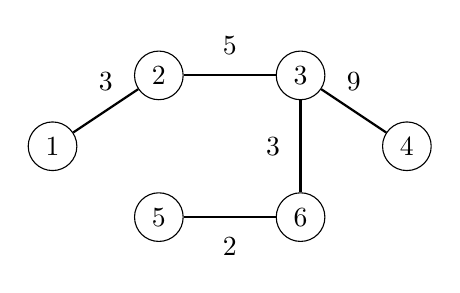
\begin{tikzpicture}[scale=0.9]
\node[draw, circle] (1) at (1.5,2) {$1$};
\node[draw, circle] (2) at (3,3) {$2$};
\node[draw, circle] (3) at (5,3) {$3$};
\node[draw, circle] (4) at (6.5,2) {$4$};
\node[draw, circle] (5) at (3,1) {$5$};
\node[draw, circle] (6) at (5,1) {$6$};
\path[draw,thick,-] (1) -- node[font=\small,label=above:3] {} (2);
\path[draw,thick,-] (2) -- node[font=\small,label=above:5] {} (3);
\path[draw,thick,-] (3) -- node[font=\small,label=above:9] {} (4);
\path[draw,thick,-] (5) -- node[font=\small,label=below:2] {} (6);
\path[draw,thick,-] (3) -- node[font=\small,label=left:3] {} (6);
\end{tikzpicture}
\end{center}

وزن یک درخت فراگیر برابر مجموع وزن یال‌های آن است.
برای مثال، وزن درخت فراگیر بالا $3+5+9+3+2=22$ است.

\index{درخت فراگیر کمینه}

یک \key{درخت فراگیر کمینه} درخت فراگیری است که وزن آن تا حد امکان کمینه باشد.
وزن درخت فراگیر کمینه برای گراف مثال برابر ۲۰ است، و چنین درختی می‌تواند به صورت زیر ساخته شود:

\begin{center}
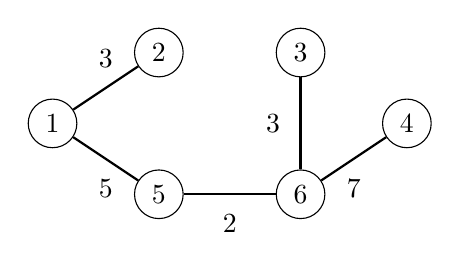
\begin{tikzpicture}[scale=0.9]
\node[draw, circle] (1) at (1.5,2) {$1$};
\node[draw, circle] (2) at (3,3) {$2$};
\node[draw, circle] (3) at (5,3) {$3$};
\node[draw, circle] (4) at (6.5,2) {$4$};
\node[draw, circle] (5) at (3,1) {$5$};
\node[draw, circle] (6) at (5,1) {$6$};

\path[draw,thick,-] (1) -- node[font=\small,label=above:3] {} (2);
\path[draw,thick,-] (1) -- node[font=\small,label=below:5] {} (5);
\path[draw,thick,-] (5) -- node[font=\small,label=below:2] {} (6);
\path[draw,thick,-] (6) -- node[font=\small,label=below:7] {} (4);
\path[draw,thick,-] (3) -- node[font=\small,label=left:3] {} (6);
\end{tikzpicture}
\end{center}

\index{درخت فراگیر بیشینه}

به روشی مشابه، یک \key{درخت فراگیر بیشینه} درختی فراگیر است که وزن آن تا حد امکان بیشینه باشد.
وزن یک درخت فراگیر بیشینه برای گراف نمونه برابر ۳۲ است:

\begin{center}
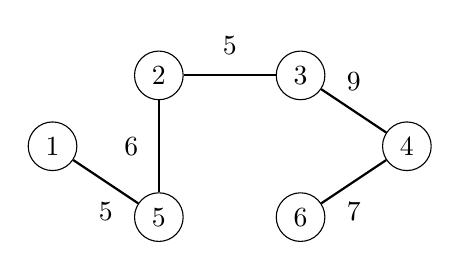
\begin{tikzpicture}[scale=0.9]
\node[draw, circle] (1) at (1.5,2) {$1$};
\node[draw, circle] (2) at (3,3) {$2$};
\node[draw, circle] (3) at (5,3) {$3$};
\node[draw, circle] (4) at (6.5,2) {$4$};
\node[draw, circle] (5) at (3,1) {$5$};
\node[draw, circle] (6) at (5,1) {$6$};
\path[draw,thick,-] (2) -- node[font=\small,label=above:5] {} (3);
\path[draw,thick,-] (3) -- node[font=\small,label=above:9] {} (4);
\path[draw,thick,-] (1) -- node[font=\small,label=below:5] {} (5);
\path[draw,thick,-] (6) -- node[font=\small,label=below:7] {} (4);
\path[draw,thick,-] (2) -- node[font=\small,label=left:6] {} (5);
\end{tikzpicture}
\end{center}

توجه داشته باشید یک گراف ممکن است چندین درخت فراگیر کمینه و بیشینه داشته باشد؛ بنابراین درخت‌ها یکتا نیستند.

مشخص شده روش‌های حریصانه متعددی برای ساخت درخت‌های فراگیر کمینه و بیشینه وجود دارد.
در این فصل، دو الگوریتم را بررسی می‌کنیم که یال‌های گراف را بر اساس وزن پردازش می‌کنند.
تمرکز ما روی یافتن درخت‌های فراگیر کمینه است، اما همین الگوریتم‌ها با پردازش معکوس یال‌ها قادر به یافتن درخت‌های فراگیر بیشینه هستند.

\section{الگوریتم کروسکال}

\index{الگوریتم کروسکال}

در \key{الگوریتم کروسکال}\footnote{این الگوریتم در سال ۱۹۵۶ توسط جی. بی. کروسکال منتشر شد \cite{kru56}.}، درخت فراگیر اولیه فقط شامل رأس‌های گراف است و هیچ یالی ندارد.
سپس الگوریتم یال‌ها را بر اساس وزن بررسی می‌کند و هر بار یالی را که دوری نسازد به درخت اضافه می‌کند.

الگوریتم مؤلفه‌های درخت را نگهداری می‌کند.
در ابتدا، هر رأس گراف متعلق به یک مؤلفه جداگانه است.
هرگاه یالی به درخت اضافه شود، دو مؤلفه ترکیب می‌شوند.
در نهایت، همه رأس‌ها عضو یک مؤلفه یکسان می‌شوند و درخت فراگیر کمینه پیدا می‌شود.

\subsubsection{مثال}

\begin{samepage}
نحوه پردازش گراف زیر توسط الگوریتم کروسکال را بررسی می‌کنیم:
\begin{center}
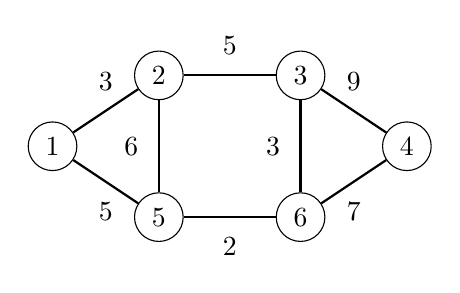
\begin{tikzpicture}[scale=0.9]
\node[draw, circle] (1) at (1.5,2) {$1$};
\node[draw, circle] (2) at (3,3) {$2$};
\node[draw, circle] (3) at (5,3) {$3$};
\node[draw, circle] (4) at (6.5,2) {$4$};
\node[draw, circle] (5) at (3,1) {$5$};
\node[draw, circle] (6) at (5,1) {$6$};
\path[draw,thick,-] (1) -- node[font=\small,label=above:3] {} (2);
\path[draw,thick,-] (2) -- node[font=\small,label=above:5] {} (3);
\path[draw,thick,-] (3) -- node[font=\small,label=above:9] {} (4);
\path[draw,thick,-] (1) -- node[font=\small,label=below:5] {} (5);
\path[draw,thick,-] (5) -- node[font=\small,label=below:2] {} (6);
\path[draw,thick,-] (6) -- node[font=\small,label=below:7] {} (4);
\path[draw,thick,-] (2) -- node[font=\small,label=left:6] {} (5);
\path[draw,thick,-] (3) -- node[font=\small,label=left:3] {} (6);
\end{tikzpicture}
\end{center}
\end{samepage}

\begin{samepage}
گام نخست الگوریتم، مرتب‌سازی یال‌ها به ترتیب صعودی وزن آن‌ها است.
نتیجه، فهرست زیر است:

\begin{tabular}{ll}
\\
یال & وزن \\
\hline
5--6 & 2 \\
1--2 & 3 \\
3--6 & 3 \\
1--5 & 5 \\
2--3 & 5 \\
2--5 & 6 \\
4--6 & 7 \\
3--4 & 9 \\
\\
\end{tabular}
\end{samepage}

سپس الگوریتم فهرست را پیمایش کرده و هر یال را در صورتی که دو مؤلفه مجزا را به هم متصل کند، به درخت اضافه می‌کند.

در ابتدا، هر رأس در مؤلفه اختصاصی خود قرار دارد:

\begin{center}
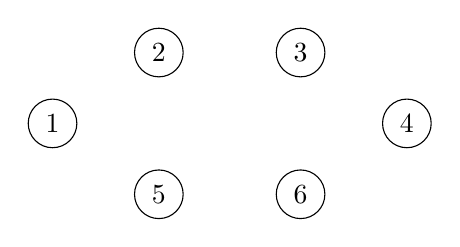
\begin{tikzpicture}[scale=0.9]
\node[draw, circle] (1) at (1.5,2) {$1$};
\node[draw, circle] (2) at (3,3) {$2$};
\node[draw, circle] (3) at (5,3) {$3$};
\node[draw, circle] (4) at (6.5,2) {$4$};
\node[draw, circle] (5) at (3,1) {$5$};
\node[draw, circle] (6) at (5,1) {$6$};
%\path[draw,thick,-] (1) -- node[font=\small,label=above:3] {} (2);
%\path[draw,thick,-] (2) -- node[font=\small,label=above:5] {} (3);
%\path[draw,thick,-] (3) -- node[font=\small,label=above:9] {} (4);
%\path[draw,thick,-] (1) -- node[font=\small,label=below:5] {} (5);
%\path[draw,thick,-] (5) -- node[font=\small,label=below:2] {} (6);
%\path[draw,thick,-] (6) -- node[font=\small,label=below:7] {} (4);
%\path[draw,thick,-] (2) -- node[font=\small,label=left:6] {} (5);
%\path[draw,thick,-] (3) -- node[font=\small,label=left:3] {} (6);
\end{tikzpicture}
\end{center}
نخستین یالی که به درخت افزوده می‌شود یال 5--6 است که با ادغام دو مؤلفه $\{5\}$ و $\{6\}$، مؤلفه $\{5,6\}$ را می‌سازد:

\begin{center}
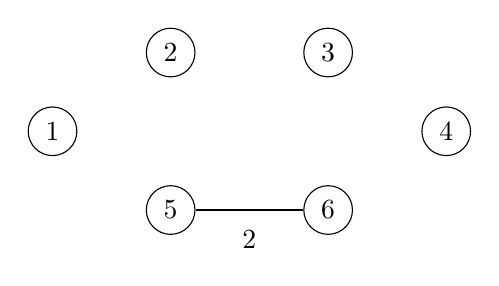
\begin{tikzpicture}
\node[draw, circle] (1) at (1.5,2) {$1$};
\node[draw, circle] (2) at (3,3) {$2$};
\node[draw, circle] (3) at (5,3) {$3$};
\node[draw, circle] (4) at (6.5,2) {$4$};
\node[draw, circle] (5) at (3,1) {$5$};
\node[draw, circle] (6) at (5,1) {$6$};

%\path[draw,thick,-] (1) -- node[font=\small,label=above:3] {} (2);
%\path[draw,thick,-] (2) -- node[font=\small,label=above:5] {} (3);
%\path[draw,thick,-] (3) -- node[font=\small,label=above:9] {} (4);
%\path[draw,thick,-] (1) -- node[font=\small,label=below:5] {} (5);
\path[draw,thick,-] (5) -- node[font=\small,label=below:2] {} (6);
%\path[draw,thick,-] (6) -- node[font=\small,label=below:7] {} (4);
%\path[draw,thick,-] (2) -- node[font=\small,label=left:6] {} (5);
%\path[draw,thick,-] (3) -- node[font=\small,label=left:3] {} (6);
\end{tikzpicture}
\end{center}
پس از آن، یال‌های 1--2، 3--6 و 1--5 به شکل مشابه اضافه می‌شوند:

\begin{center}
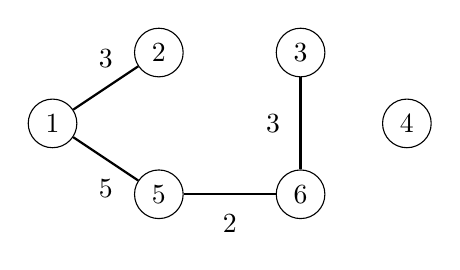
\begin{tikzpicture}[scale=0.9]
\node[draw, circle] (1) at (1.5,2) {$1$};
\node[draw, circle] (2) at (3,3) {$2$};
\node[draw, circle] (3) at (5,3) {$3$};
\node[draw, circle] (4) at (6.5,2) {$4$};
\node[draw, circle] (5) at (3,1) {$5$};
\node[draw, circle] (6) at (5,1) {$6$};

\path[draw,thick,-] (1) -- node[font=\small,label=above:3] {} (2);
%\path[draw,thick,-] (2) -- node[font=\small,label=above:5] {} (3);
%\path[draw,thick,-] (3) -- node[font=\small,label=above:9] {} (4);
\path[draw,thick,-] (1) -- node[font=\small,label=below:5] {} (5);
\path[draw,thick,-] (5) -- node[font=\small,label=below:2] {} (6);
%\path[draw,thick,-] (6) -- node[font=\small,label=below:7] {} (4);
%\path[draw,thick,-] (2) -- node[font=\small,label=left:6] {} (5);
\path[draw,thick,-] (3) -- node[font=\small,label=left:3] {} (6);
\end{tikzpicture}
\end{center}

پس از این مراحل، بیشتر مولفه‌ها ادغام شده‌اند
و دو مولفه در درخت وجود دارد:
$\{1,2,3,5,6\}$ و $\{4\}$.

یال بعدی فهرست یال 2--3 است،
اما به درخت اضافه نمی‌شود، چون
راس‌های ۲ و ۳ از قبل در یک مولفه‌اند.
به همین دلیل، یال 2--5 نیز به درخت اضافه نخواهد شد.

\begin{samepage}
در نهایت، یال 4--6 به درخت اضافه می‌شود:

\begin{center}
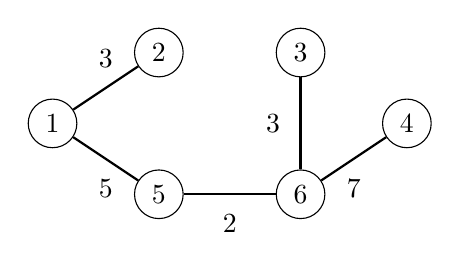
\begin{tikzpicture}[scale=0.9]
\node[draw, circle] (1) at (1.5,2) {$1$};
\node[draw, circle] (2) at (3,3) {$2$};
\node[draw, circle] (3) at (5,3) {$3$};
\node[draw, circle] (4) at (6.5,2) {$4$};
\node[draw, circle] (5) at (3,1) {$5$};
\node[draw, circle] (6) at (5,1) {$6$};

\path[draw,thick,-] (1) -- node[font=\small,label=above:3] {} (2);
%\path[draw,thick,-] (2) -- node[font=\small,label=above:5] {} (3);
%\path[draw,thick,-] (3) -- node[font=\small,label=above:9] {} (4);
\path[draw,thick,-] (1) -- node[font=\small,label=below:5] {} (5);
\path[draw,thick,-] (5) -- node[font=\small,label=below:2] {} (6);
\path[draw,thick,-] (6) -- node[font=\small,label=below:7] {} (4);
%\path[draw,thick,-] (2) -- node[font=\small,label=left:6] {} (5);
\path[draw,thick,-] (3) -- node[font=\small,label=left:3] {} (6);
\end{tikzpicture}
\end{center}
\end{samepage}

پس از این، الگوریتم یال جدیدی اضافه نخواهد کرد، زیرا گراف همبند است
و بین هر دو راس یک مسیر وجود دارد.
گراف حاصل یک درخت فراگیر کمینه
با وزن $2+3+3+5+7=20$ است.

\subsubsection{چرا این روش کار می‌کند؟}

این پرسش خوبی است که چرا الگوریتم کروسکال به درستی کار می‌کند.
چرا راهبرد حریصانه تضمین می‌کند که
یک درخت فراگیر کمینه پیدا خواهیم کرد؟

بیایید بررسی کنیم چه اتفاقی می‌افتد اگر یال با کمترین وزن گراف،
در درخت فراگیر \emph{قرار نگیرد}.
برای نمونه، فرض کنید یک درخت فراگیر
برای گراف پیشین شامل یال با کمترین وزن یعنی 5--6 نباشد.
ساختار دقیق چنین درخت فراگیری را نمی‌دانیم،
اما در هر صورت باید یال‌هایی داشته باشد.
فرض کنید درخت به شکل زیر باشد:

\begin{center}
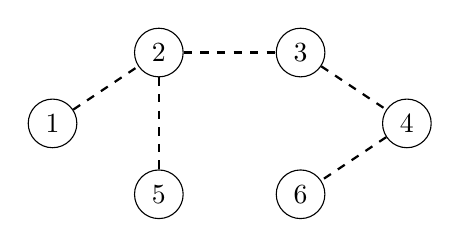
\begin{tikzpicture}[scale=0.9]
\node[draw, circle] (1) at (1.5,2) {$1$};
\node[draw, circle] (2) at (3,3) {$2$};
\node[draw, circle] (3) at (5,3) {$3$};
\node[draw, circle] (4) at (6.5,2) {$4$};
\node[draw, circle] (5) at (3,1) {$5$};
\node[draw, circle] (6) at (5,1) {$6$};

\path[draw,thick,-,dashed] (1) -- (2);
\path[draw,thick,-,dashed] (2) -- (5);
\path[draw,thick,-,dashed] (2) -- (3);
\path[draw,thick,-,dashed] (3) -- (4);
\path[draw,thick,-,dashed] (4) -- (6);
\end{tikzpicture}
\end{center}

اما درخت فوق نمی‌تواند درخت فراگیر کمینه برای گراف باشد. دلیل این است که می‌توانیم یالی را از درخت حذف کرده و یال با کمینه وزن یعنی 5--6 را جایگزین آن کنیم. این کار درختی فراگیر با وزن \emph{کمتر} تولید می‌کند:

\begin{center}
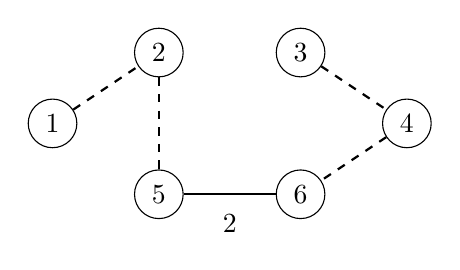
\begin{tikzpicture}[scale=0.9]
\node[draw, circle] (1) at (1.5,2) {$1$};
\node[draw, circle] (2) at (3,3) {$2$};
\node[draw, circle] (3) at (5,3) {$3$};
\node[draw, circle] (4) at (6.5,2) {$4$};
\node[draw, circle] (5) at (3,1) {$5$};
\node[draw, circle] (6) at (5,1) {$6$};

\path[draw,thick,-,dashed] (1) -- (2);
\path[draw,thick,-,dashed] (2) -- (5);
\path[draw,thick,-,dashed] (3) -- (4);
\path[draw,thick,-,dashed] (4) -- (6);
\path[draw,thick,-] (5) -- node[font=\small,label=below:2] {} (6);
\end{tikzpicture}
\end{center}

به همین دلیل، همواره بهینه است که یال با کمترین وزن برای ساخت درخت فراگیر کمینه به درخت اضافه شود. با استدلالی مشابه می‌توان نشان داد اضافه کردن یال بعدی بر اساس ترتیب وزن به درخت نیز بهینه است، و به همین ترتیب تا انتها ادامه می‌یابد. بنابراین الگوریتم کروسکال به درستی کار می‌کند و همواره یک درخت فراگیر کمینه می‌سازد.

\subsubsection{پیاده‌سازی}

در پیاده‌سازی الگوریتم کروسکال، استفاده از نمایش فهرست یال‌ها برای گراف مناسب است. گام اول الگوریتم، یال‌های فهرست را در زمان $O(m \log m)$ مرتب می‌کند. سپس گام دوم الگوریتم، درخت فراگیر کمینه را به شکل زیر می‌سازد:

\begin{lstlisting}
for (...) {
  if (!same(a,b)) unite(a,b);
}
\end{lstlisting}

حلقه روی یال‌های فهرست پیمایش کرده و هر بار یال $a$--$b$ را پردازش می‌کند که در آن $a$ و $b$ دو رأس هستند. دو تابع مورد نیاز است: تابع \texttt{same} بررسی می‌کند آیا $a$ و $b$ در یک مولفه هستند، و تابع \texttt{unite} مولفه‌های شامل $a$ و $b$ را ادغام می‌کند.

مسئله، پیاده‌سازی کارآمد توابع \texttt{same} و \texttt{unite} است. یک روش، پیاده‌سازی \texttt{same} با پیمایش گراف و بررسی وجود مسیر بین $a$ و $b$ است. ولی پیچیدگی زمانی چنین تابعی $O(n+m)$ خواهد بود و الگوریتم کند می‌شود، زیرا \texttt{same} به ازای هر یال در گراف فراخوانی خواهد شد.

این مسئله را با ساختار مجموعه‌های مجزا (union-find) حل می‌کنیم که هر دو تابع را در زمان $O(\log n)$ اجرا می‌کند. بدین ترتیب پیچیدگی زمانی الگوریتم کروسکال پس از مرتب‌سازی فهرست یال‌ها، $O(m \log n)$ خواهد بود.

\section{ساختار مجموعه‌های مجزا}

\index{ساختار مجموعه‌های مجزا}

یک \key{ساختمان داده مجموعه‌های مجزا} (union-find)
مجموعه‌ای از دسته‌ها را نگهداری می‌کند.
مجموعه‌ها مجزا هستند، بنابراین هیچ عنصری
در بیش از یک مجموعه وجود ندارد.
دو عملیات با زمان $O(\log n)$ پشتیبانی می‌شوند:
عملیات \texttt{unite} دو مجموعه را ادغام می‌کند،
و عملیات \texttt{find} نماینده‌ی مجموعه‌ای
شامل عنصر داده‌شده را می‌یابد\footnote{ساختار ارائه‌شده در اینجا
در سال ۱۹۷۱ توسط جی. دی. هاپ‌کرافت و جی. دی. اولمن معرفی شد \cite{hop71}.
سپس، در ۱۹۷۵، آر. ای. تارجان نسخه‌ای پیشرفته‌تر
از این ساختار را بررسی کرد \cite{tar75} که امروزه در کتاب‌های مرجع الگوریتم بررسی می‌شود.}.

\subsubsection{ساختار}

در ساختار مجموعه‌های مجزا، یک عضو در هر مجموعه
نماینده‌ی مجموعه است،
و زنجیره‌ای از هر عضو دیگر مجموعه به سمت نماینده وجود دارد.
برای مثال فرض کنید مجموعه‌ها
$\{1,4,7\}$، $\{5\}$ و $\{2,3,6,8\}$ باشند:
\begin{center}
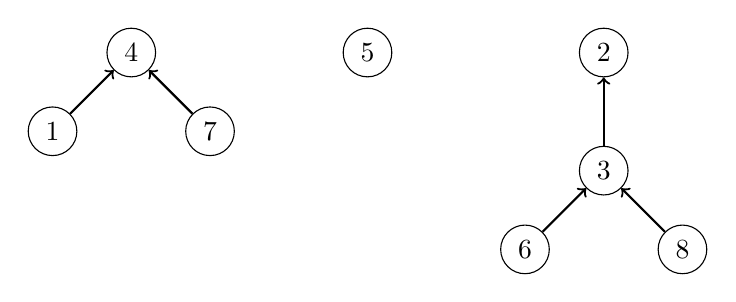
\begin{tikzpicture}
\node[draw, circle] (1) at (0,-1) {$1$};
\node[draw, circle] (2) at (7,0) {$2$};
\node[draw, circle] (3) at (7,-1.5) {$3$};
\node[draw, circle] (4) at (1,0) {$4$};
\node[draw, circle] (5) at (4,0) {$5$};
\node[draw, circle] (6) at (6,-2.5) {$6$};
\node[draw, circle] (7) at (2,-1) {$7$};
\node[draw, circle] (8) at (8,-2.5) {$8$};

\path[draw,thick,->] (1) -- (4);
\path[draw,thick,->] (7) -- (4);

\path[draw,thick,->] (3) -- (2);
\path[draw,thick,->] (6) -- (3);
\path[draw,thick,->] (8) -- (3);

\end{tikzpicture}
\end{center}
در این حالت، نمایندگان مجموعه‌ها
۴، ۵ و ۲ هستند.
می‌توان نماینده‌ی هر عضو را
با پیمایش زنجیره‌ی شروع‌شده از آن عضو پیدا کرد.
برای نمونه، عنصر ۲ نماینده‌ی عنصر ۶ است، زیرا
زنجیره‌ی $6 \rightarrow 3 \rightarrow 2$ را دنبال می‌کنیم.
دو عنصر متعلق به یک مجموعه‌اند دقیقاً اگر
نمایندگان یکسانی داشته باشند.

دو مجموعه را می‌توان با متصل کردن
نماینده‌ی یک مجموعه به نماینده‌ی مجموعه‌ی دیگر
ادغام کرد.
برای مثال، مجموعه‌های
$\{1,4,7\}$ و $\{2,3,6,8\}$
به این شکل ادغام می‌شوند:
\begin{center}
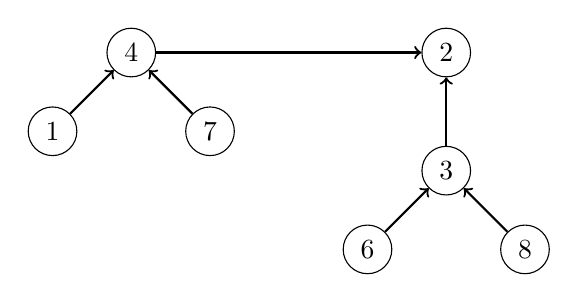
\begin{tikzpicture}
\node[draw, circle] (1) at (2,-1) {$1$};
\node[draw, circle] (2) at (7,0) {$2$};
\node[draw, circle] (3) at (7,-1.5) {$3$};
\node[draw, circle] (4) at (3,0) {$4$};
\node[draw, circle] (6) at (6,-2.5) {$6$};
\node[draw, circle] (7) at (4,-1) {$7$};
\node[draw, circle] (8) at (8,-2.5) {$8$};

\path[draw,thick,->] (1) -- (4);
\path[draw,thick,->] (7) -- (4);

\path[draw,thick,->] (3) -- (2);
\path[draw,thick,->] (6) -- (3);
\path[draw,thick,->] (8) -- (3);

\path[draw,thick,->] (4) -- (2);
\end{tikzpicture}
\end{center}

مجموعه حاصل شامل اعضای
$\{1,2,3,4,6,7,8\}$ است.
از این پس، عنصر ۲ نماینده‌ی کل مجموعه است
و نماینده‌ی پیشین ۴ به عنصر ۲ اشاره دارد.

کارایی ساختار مجموعه‌های مجزا (union-find) به نحوه
ادغام مجموعه‌ها بستگی دارد.
می‌توان از یک استراتژی ساده پیروی کرد:
همیشه نماینده مجموعه \emph{کوچک‌تر} را به نماینده مجموعه \emph{بزرگ‌تر}
متصل کنید (یا اگر مجموعه‌ها هم‌اندازه باشند،
می‌توان انتخابی دلخواه داشت).
با این روش، طول هر زنجیره $O(\log n)$ خواهد بود،
بنابراین می‌توان نماینده هر عنصر را با دنبال کردن
زنجیره مربوطه به طور کارآمد پیدا کرد.

\subsubsection{پیاده‌سازی}

ساختار مجموعه‌های مجزا را می‌توان
با آرایه‌ها پیاده‌سازی کرد.
در پیاده‌سازی زیر،
آرایه \texttt{link} برای هر عنصر،
عنصر بعدی در زنجیره یا در صورت نماینده بودن،
خود آن عنصر را نگه‌داری می‌کند،
و آرایه \texttt{size} برای هر نماینده،
اندازه مجموعه متناظر را نشان می‌دهد.

در ابتدا، هر عنصر به یک مجموعه مجزا تعلق دارد:
\begin{lstlisting}
for (int i = 1; i <= n; i++) link[i] = i;
for (int i = 1; i <= n; i++) size[i] = 1;
\end{lstlisting}

تابع \texttt{find} نماینده
عنصر $x$ را برمی‌گرداند.
نماینده را می‌توان با دنبال کردن
زنجیره‌ای که از $x$ شروع می‌شود پیدا کرد.

\begin{lstlisting}
int find(int x) {
    while (x != link[x]) x = link[x];
    return x;
}
\end{lstlisting}

تابع \texttt{same} بررسی می‌کند
که آیا عناصر $a$ و $b$ به یک مجموعه تعلق دارند یا خیر.
این کار را می‌توان به سادگی با استفاده از
تابع \texttt{find} انجام داد:

\begin{lstlisting}
bool same(int a, int b) {
    return find(a) == find(b);
}
\end{lstlisting}

\begin{samepage}
تابع \texttt{unite} مجموعه‌های شامل
عناصر $a$ و $b$ را ادغام می‌کند
(عناصر باید در مجموعه‌های متفاوتی باشند).
تابع ابتدا نمایندگان مجموعه‌ها را پیدا می‌کند
و سپس مجموعه کوچک‌تر را به مجموعه بزرگ‌تر متصل می‌کند.

\begin{lstlisting}
void unite(int a, int b) {
    a = find(a);
    b = find(b);
    if (size[a] < size[b]) swap(a,b);
    size[a] += size[b];
    link[b] = a;
}
\end{lstlisting}
\end{samepage}

پیچیدگی زمانی تابع \texttt{find}
با فرض اینکه طول هر زنجیره $O(\log n)$ است،
برابر $O(\log n)$ خواهد بود.
در این حالت، توابع \texttt{same} و \texttt{unite} نیز
در زمان $O(\log n)$ اجرا می‌شوند.
تابع \texttt{unite} تضمین می‌کند که با اتصال
مجموعه کوچک‌تر به مجموعه بزرگ‌تر،
طول هر زنجیره $O(\log n)$ باقی بماند.

\section{الگوریتم پریم}

\index{الگوریتم پریم}

\key{الگوریتم پریم}\footnote{این الگوریتم به نام
آر. سی. پریم (R. C. Prim) که آن را در سال ۱۹۵۷ منتشر کرد \cite{pri57}
نام‌گذاری شده است. با این حال، همین الگوریتم پیش‌تر در سال ۱۹۳۰
توسط وی. یارنیک (V. Jarník) کشف شده بود.} روشی جایگزین
برای یافتن درخت پوشای کمینه است.
الگوریتم ابتدا یک رأس دلخواه را
به درخت اضافه می‌کند.
پس از آن، الگوریتم همواره یالی با کمترین وزن را
انتخاب می‌کند که یک رأس جدید را به درخت اضافه کند.
در نهایت، همه رئوس به درخت اضافه می‌شوند
و یک درخت پوشای کمینه حاصل می‌شود.

الگوریتم پریم شبیه الگوریتم دایکسترا است. تفاوت این است که الگوریتم دایکسترا همیشه یالی را برمی‌گزیند که فاصله‌اش از گره آغازین کمینه باشد، ولی الگوریتم پریم کم‌وزن‌ترین یالی را برمی‌گزیند که گرهی تازه به درخت می‌افزاید.

\subsubsection{مثال}

چگونگی کارکرد الگوریتم پریم در گراف زیر را بررسی می‌کنیم:

\begin{center}
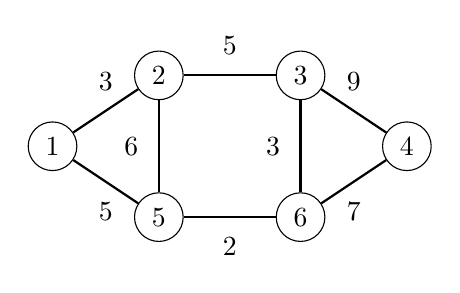
\begin{tikzpicture}[scale=0.9]
\node[draw, circle] (1) at (1.5,2) {$1$};
\node[draw, circle] (2) at (3,3) {$2$};
\node[draw, circle] (3) at (5,3) {$3$};
\node[draw, circle] (4) at (6.5,2) {$4$};
\node[draw, circle] (5) at (3,1) {$5$};
\node[draw, circle] (6) at (5,1) {$6$};
\path[draw,thick,-] (1) -- node[font=\small,label=above:3] {} (2);
\path[draw,thick,-] (2) -- node[font=\small,label=above:5] {} (3);
\path[draw,thick,-] (3) -- node[font=\small,label=above:9] {} (4);
\path[draw,thick,-] (1) -- node[font=\small,label=below:5] {} (5);
\path[draw,thick,-] (5) -- node[font=\small,label=below:2] {} (6);
\path[draw,thick,-] (6) -- node[font=\small,label=below:7] {} (4);
\path[draw,thick,-] (2) -- node[font=\small,label=left:6] {} (5);
\path[draw,thick,-] (3) -- node[font=\small,label=left:3] {} (6);

%\path[draw=red,thick,-,line width=2pt] (5) -- (6);
\end{tikzpicture}
\end{center}
در ابتدا، هیچ یالی بین رأس‌ها وجود ندارد:
\begin{center}
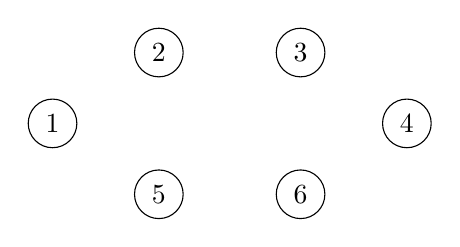
\begin{tikzpicture}[scale=0.9]
\node[draw, circle] (1) at (1.5,2) {$1$};
\node[draw, circle] (2) at (3,3) {$2$};
\node[draw, circle] (3) at (5,3) {$3$};
\node[draw, circle] (4) at (6.5,2) {$4$};
\node[draw, circle] (5) at (3,1) {$5$};
\node[draw, circle] (6) at (5,1) {$6$};
%\path[draw,thick,-] (1) -- node[font=\small,label=above:3] {} (2);
%\path[draw,thick,-] (2) -- node[font=\small,label=above:5] {} (3);
%\path[draw,thick,-] (3) -- node[font=\small,label=above:9] {} (4);
%\path[draw,thick,-] (1) -- node[font=\small,label=below:5] {} (5);
%\path[draw,thick,-] (5) -- node[font=\small,label=below:2] {} (6);
%\path[draw,thick,-] (6) -- node[font=\small,label=below:7] {} (4);
%\path[draw,thick,-] (2) -- node[font=\small,label=left:6] {} (5);
%\path[draw,thick,-] (3) -- node[font=\small,label=left:3] {} (6);
\end{tikzpicture}
\end{center}
یک رأس دلخواه می‌تواند رأس آغازین باشد،
پس رأس 1 را انتخاب می‌کنیم.
ابتدا، رأس 2 را که با یالی به وزن 3 متصل است
اضافه می‌کنیم:
\begin{center}
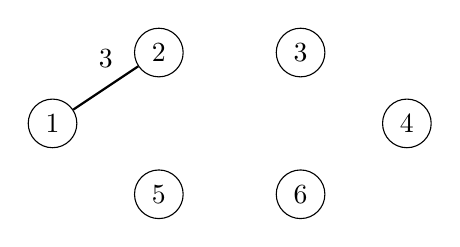
\begin{tikzpicture}[scale=0.9]
\node[draw, circle] (1) at (1.5,2) {$1$};
\node[draw, circle] (2) at (3,3) {$2$};
\node[draw, circle] (3) at (5,3) {$3$};
\node[draw, circle] (4) at (6.5,2) {$4$};
\node[draw, circle] (5) at (3,1) {$5$};
\node[draw, circle] (6) at (5,1) {$6$};
\path[draw,thick,-] (1) -- node[font=\small,label=above:3] {} (2);
%\path[draw,thick,-] (2) -- node[font=\small,label=above:5] {} (3);
%\path[draw,thick,-] (3) -- node[font=\small,label=above:9] {} (4);
%\path[draw,thick,-] (1) -- node[font=\small,label=below:5] {} (5);
%\path[draw,thick,-] (5) -- node[font=\small,label=below:2] {} (6);
%\path[draw,thick,-] (6) -- node[font=\small,label=below:7] {} (4);
%\path[draw,thick,-] (2) -- node[font=\small,label=left:6] {} (5);
%\path[draw,thick,-] (3) -- node[font=\small,label=left:3] {} (6);
\end{tikzpicture}
\end{center}

پس از این، دو یال با وزن 5 وجود دارد،
بنابراین می‌توانیم رأس 3 یا رأس 5 را به درخت اضافه کنیم.
ابتدا رأس 3 را اضافه می‌کنیم:
\begin{center}
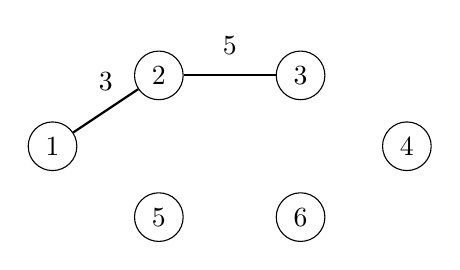
\begin{tikzpicture}[scale=0.9]
\node[draw, circle] (1) at (1.5,2) {$1$};
\node[draw, circle] (2) at (3,3) {$2$};
\node[draw, circle] (3) at (5,3) {$3$};
\node[draw, circle] (4) at (6.5,2) {$4$};
\node[draw, circle] (5) at (3,1) {$5$};
\node[draw, circle] (6) at (5,1) {$6$};
\path[draw,thick,-] (1) -- node[font=\small,label=above:3] {} (2);
\path[draw,thick,-] (2) -- node[font=\small,label=above:5] {} (3);
%\path[draw,thick,-] (3) -- node[font=\small,label=above:9] {} (4);
%\path[draw,thick,-] (1) -- node[font=\small,label=below:5] {} (5);
%\path[draw,thick,-] (5) -- node[font=\small,label=below:2] {} (6);
%\path[draw,thick,-] (6) -- node[font=\small,label=below:7] {} (4);
%\path[draw,thick,-] (2) -- node[font=\small,label=left:6] {} (5);
%\path[draw,thick,-] (3) -- node[font=\small,label=left:3] {} (6);
\end{tikzpicture}
\end{center}

\begin{samepage}
فرایند تا زمانی که تمام رأس‌ها به درخت اضافه شوند ادامه می‌یابد:
\begin{center}
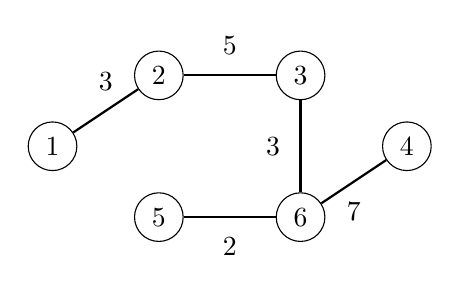
\begin{tikzpicture}[scale=0.9]
\node[draw, circle] (1) at (1.5,2) {$1$};
\node[draw, circle] (2) at (3,3) {$2$};
\node[draw, circle] (3) at (5,3) {$3$};
\node[draw, circle] (4) at (6.5,2) {$4$};
\node[draw, circle] (5) at (3,1) {$5$};
\node[draw, circle] (6) at (5,1) {$6$};
\path[draw,thick,-] (1) -- node[font=\small,label=above:3] {} (2);
\path[draw,thick,-] (2) -- node[font=\small,label=above:5] {} (3);
%\path[draw,thick,-] (3) -- node[font=\small,label=above:9] {} (4);
%\path[draw,thick,-] (1) -- node[font=\small,label=below:5] {} (5);
\path[draw,thick,-] (5) -- node[font=\small,label=below:2] {} (6);
\path[draw,thick,-] (6) -- node[font=\small,label=below:7] {} (4);
%\path[draw,thick,-] (2) -- node[font=\small,label=left:6] {} (5);
\path[draw,thick,-] (3) -- node[font=\small,label=left:3] {} (6);
\end{tikzpicture}
\end{center}
\end{samepage}

\subsubsection{پیاده‌سازی}

مشابه الگوریتم دایکسترا، الگوریتم پریم را می‌توان با استفاده از یک صف اولویت‌دار بهینه‌سازی و پیاده‌سازی کرد.
صف اولویت‌دار باید شامل تمام رأس‌هایی باشد که می‌توان آن‌ها را با یک یال به مؤلفه فعلی متصل کرد، مرتب‌شده به صورت صعودی بر اساس وزن یال‌های متناظر.

پیچیدگی زمانی الگوریتم پریم $O(n + m \log m)$ است که با پیچیدگی زمانی الگوریتم دایکسترا برابر است.
در عمل، هر دو الگوریتم پریم و کروسکال کارآمد هستند و انتخاب الگوریتم سلیقه‌ای است.
با این حال، اکثر برنامه‌نویسان رقابتی از الگوریتم کروسکال استفاده می‌کنند.